\documentclass[reprint,aps,prresearch]{revtex4-2}
\usepackage{amsmath,amssymb,graphicx,booktabs}
\begin{document}
\title{Outcome-Trajectory Independence of Occupied-Frame Chern-State Preparation}
\author{Numerical validation campaign}
\date{\today}
\maketitle
\section{Protocol}
Ten independent Born-outcome trajectories share one random-pure initial state and one frozen random site schedule. The controller uses $N_x=N_y=16$, 32 cycles, $n_{\rm shell}=1$, domain wall off, $\alpha=1$, perfect correction, and no postselection. The independent sampling unit is one complete outcome trajectory conditional on the fixed initial state and schedule. Pairwise distances are not treated as independent samples.

Evolution is performed directly on the occupied frame. Physical projectors are reconstructed only after the trajectories finish, for diagnostic comparison. A covariance replay of trajectory zero gives maximum relative error 7.581e-14 and maximum element error 2.386e-13.

\section{Classification}
The campaign classification is \texttt{trajectory\_dependent\_at\_32\_cycles}. The exact-state gate is false, and the topology gate is false. The finite-size target marker is 0.999464968; the final ensemble mean is 0.994559377 with trajectory standard deviation 1.475e-02. The maximum final pairwise projector distance is 1.076e-01, and the final ranks are [256, 256, 258, 260, 257, 256, 256, 257, 255, 256].

\begin{figure}[t]
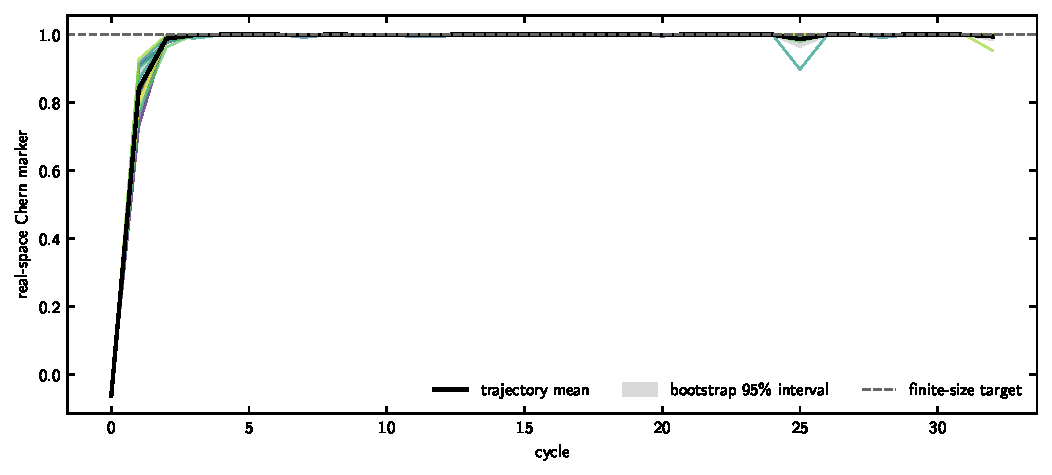
\includegraphics[width=\linewidth]{../figures/chern_trajectories.pdf}
\caption{Individual and ensemble real-space Chern-marker convergence for $S=10$ outcome trajectories. The band is a whole-trajectory bootstrap 95\% interval with 10,000 resamples.}
\end{figure}

\begin{figure}[t]
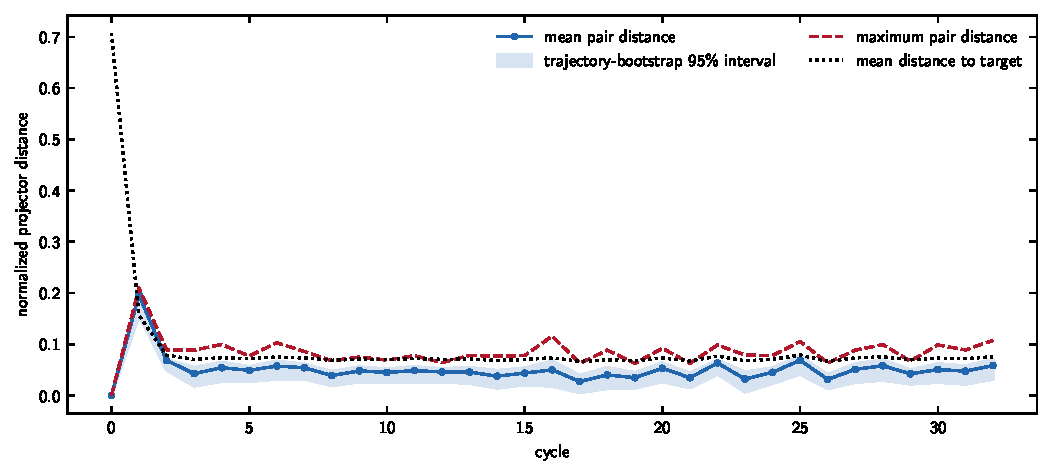
\includegraphics[width=\linewidth]{../figures/projector_distance_convergence.pdf}
\caption{Mean and maximum pairwise occupied-projector distance. The 45 pairs are dependent; uncertainty is obtained by resampling the ten trajectories.}
\end{figure}

\begin{figure}[t]
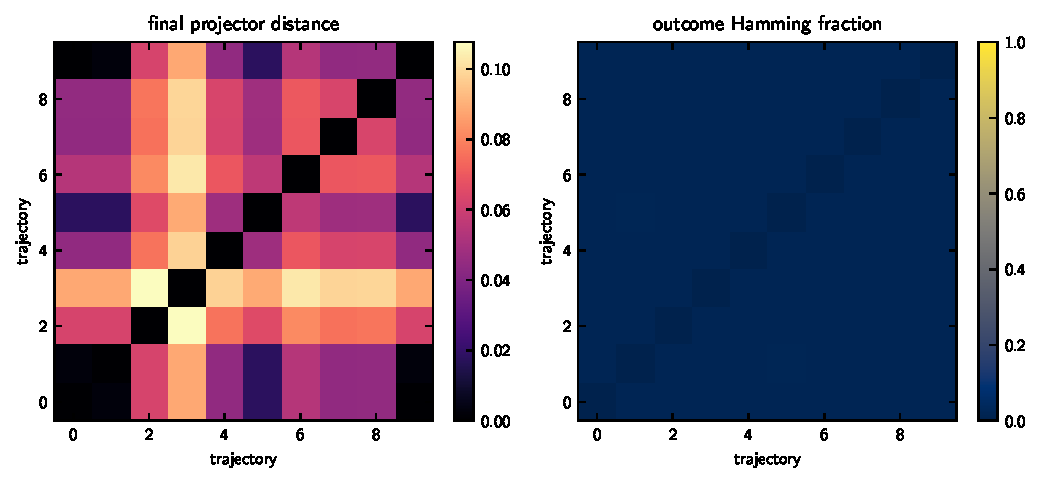
\includegraphics[width=\linewidth]{../figures/pairwise_heatmaps.pdf}
\caption{Final microscopic state separation compared with measurement-record separation.}
\end{figure}

\section{Interpretation}
Exact final-state independence would permit independently realized records to represent the same state at different boundary twists. Topology-only independence establishes a common Chern phase but does not make unrelated trajectories into one smooth Berry bundle. This experiment is conditional on one frozen site schedule and does not test schedule-to-schedule variation.
\end{document}
